\documentclass[runningheads]{llncs}

\usepackage{graphicx}
\usepackage{amsmath,amssymb}
\usepackage{graphicx}
\usepackage{algorithm}
\usepackage{algorithmic}
\usepackage[ruled,vlined]{algorithm2e}
\usepackage{float}
\usepackage{geometry}
\usepackage{url}
\usepackage{booktabs}
\usepackage[demo]{graphicx}
\usepackage{caption}
\usepackage{subcaption}
\usepackage[backend=bibtex]{biblatex}
\addbibresource{main.bib}

\title{Differential and Linear Cryptanalysis of Modular Addition}
\author{Halil \.{I}brahim Kaplan\inst{1} Ali Doğan \inst{2} Gökçe Yetişer \inst{3} }
\institute{Cryptanalsis Laboratory, Tübitak BİLGEM, Kocaeli, Turkey \\ \email{halil.kaplan@tubitak.gov.tr} \and Istanbul Settlement and Custody Bank(TAKASBANK), Istanbul, Turkey \\ \email{adogan@takasbank.com.tr
} \and Teila, Stockholm, Switzerland \\ \email{gokceyetiser@gmail.com} }

\begin{document}

\maketitle

\begin{keywords}
Linear cryptanalysis, Differential cryptanalysis, Modular addition, LAT, DDT, Carry bits, ARX ciphers
\end{keywords}

\begin{abstract}
This paper presents a comprehensive analysis of modular addition from a cryptanalytic perspective, focusing on both linear and differential cryptanalysis techniques. We examine the probability distribution of carry bits in modular addition operations and demonstrate how these probabilities affect linear approximations. The paper provides detailed algorithms for constructing Linear Approximation Tables (LAT) and Difference Distribution Tables (DDT) for modular addition operations, along with theoretical proofs and practical examples. Our analysis reveals that the probability of carry bits approaches 1/2 as the bit position increases, which significantly impacts the effectiveness of linear cryptanalysis. Furthermore, we demonstrate how to extend DDTs for larger bit sizes by leveraging smaller tables and carry bit relationships. The findings have direct implications for the cryptanalysis of ARX ciphers.
\end{abstract}

\section{Introduction}
Modular addition is a fundamental operation in many symmetric-key cryptographic algorithms, including ARX (Addition-Rotation-XOR) ciphers and others like RC5, IDEA, and SPECK. Understanding its cryptographic properties is essential for both designing secure ciphers and analyzing existing ones.

This paper focuses on two main aspects of modular addition cryptanalysis: linear cryptanalysis and differential cryptanalysis. We begin by analyzing the probability distribution of carry bits in modular addition operations, which plays a crucial role in determining the effectiveness of linear approximations. We then present methods for constructing Linear Approximation Tables (LAT) and Difference Distribution Tables (DDT) specifically for modular addition operations.

The contributions of this paper include:
\begin{itemize}
\item A detailed analysis of carry bit probability distribution in modular addition
\item Algorithms for constructing LAT and DDT for modular addition
\item Theoretical proofs of key properties affecting linear and differential cryptanalysis
\item Practical examples demonstrating the application of these techniques
\item Methods for extending DDTs to larger bit sizes using smaller tables
\end{itemize}

Our findings provide valuable insights for cryptanalysts examining algorithms that use modular addition and for cipher designers seeking to understand potential vulnerabilities in their constructions.


\section{Modular addition}

Let \( x = (x_n, \dots, x_0) \) and \( y = (y_n, \dots, y_0) \) be two \( n \)-bit strings. Let \( z = x \boxplus y \), where \( \boxplus \) denotes modular addition. We can express modular addition operation with xor using equation from \cite{Dehnavi2014} 
\begin{lemma}
    Let \( z = x \boxplus y \), where \( x = (x_{31}, \ldots, x_0) \), \( y = (y_{31}, \ldots, y_0) \), and \( z = (z_{31}, \ldots, z_0) \). Then:
    \[
    z_0 = x_0 \oplus y_0, \quad z_1 = x_1 \oplus y_1 \oplus x_0 y_0,
    \]
    and for \( 2 \leq i \leq 31 \):
    \[
    z_i = x_i \oplus y_i \oplus x_{i-1} y_{i-1} \oplus \sum_{t=0}^{i-2} x_t y_t \left( \prod_{r=t+1}^{i-1} (x_r \oplus y_r) \right)
    \]
    Each output bit \( z_i \) is thus a Boolean function of degree \( i + 1 \).
\end{lemma}

We can also use carry bits to express modular addition :
\begin{lemma}
    Let \( C_i(x, y) \) represent the carry bit propagated to the \( i \)-th bit position. For \( 0 \leq i \leq n \), the bits \( z_i \) and \( C_i \) can be computed using the following equations:
    \[
    z_i = x_i \oplus y_i \oplus C_i(x,y),
    \]
    \[
    C_i = x_i y_i \oplus C_{i-1}(x,y)(x_i \oplus y_i).
    \]
\end{lemma}


\section{Carry bit probablity distrubition}

To compute the probability distribution of the carry bit at position \( i \), we need to know the value of the carry bit at position \( i-1 \). Therefore, the probability can be analyzed under two separate cases. Let us consider the first case where the carry bit at position \( i-1 \) is 0.

\begin{table}[h]
\centering
    \begin{tabular}{ c || c | c | c | c }
        $x_i$ & 0 & 0 & 1 & 1 \\ 
        $y_i$ & 0 & 1 & 0 & 1 \\ 
        \hline
        $C_i$ & \textbf{0} & \textbf{0} & \textbf{0} & \textbf{1}    
    \end{tabular}
    \caption{$C_{i-1} = 0$}
    \label{tab:1}
\end{table}

From Table \ref{tab:1}, we observe that the carry bit at position \( i \) is 1 with probability \( \frac{1}{4} \), and 0 with probability \( \frac{3}{4} \). To complete the analysis, let us examine the second case where the carry bit at position \( i-1 \) is 1.

\begin{table}[h]
\centering
    \begin{tabular}{ c || c | c | c | c }
    $x_i$ & 0 & 0 & 1 & 1 \\ 
    $y_i$ & 0 & 1 & 0 & 1 \\ 
    \hline
    $C_i$ & \textbf{0} & \textbf{1} & \textbf{1} & \textbf{1}  
    \end{tabular}
    \caption{$C_{i-1} = 1$}
    \label{tab:2}
\end{table}

From Table \ref{tab:2}, we see that the carry bit at position \( i \) is 1 with probability \( \frac{3}{4} \), and 0 with probability \( \frac{1}{4} \). Considering both cases, the probability that \( C_i = 1 \) given the value of the previous carry bit can be expressed as:

\begin{center}
\[
\Pr[C_i = 1] = \frac{1}{4} \cdot \Pr[C_{i-1} = 0] + \frac{3}{4} \cdot \Pr[C_{i-1} = 1]
\]
\end{center}

From the recurrence above, we can intuitively observe that the probability approaches \( \frac{1}{2} \) as \( i \) increases.

\begin{center}
\begin{align*}
\Pr[C_1 = 1] &= \frac{1}{4} \\
\Pr[C_2 = 1] &= \frac{3}{8} \\
\Pr[C_3 = 1] &= \frac{7}{16} \\
\Pr[C_4 = 1] &= \frac{15}{32} \\
&\vdots
\end{align*}
\end{center}

Alternatively, we can compute the probability of the carry bit being 1 without knowing the previous carry bit explicitly.

\begin{table}[h]
\centering
    \begin{tabular}{ c || c | c | c | c }
    $x_i$ & 0 & 0 & 1 & 1 \\ 
    $y_i$ & 0 & 1 & 0 & 1 \\ 
    \hline
    $C_i$ & \textbf{0} & \textbf{?} & \textbf{?} & \textbf{1}  
    \end{tabular}
    \caption{$C_{i-1} = ?$}
    \label{tab:2}
\end{table}

In this setting, when both \( x_i \) and \( y_i \) are 0, the carry bit at position \( i \) is 0 regardless of the previous carry bit. When both are 1, the carry bit at position \( i \) is always 1. In the remaining two cases, the value of \( C_i \) depends on the previous carry bit. That is, in \( \frac{1}{4} \) of the cases, the carry bit is definitively 1, and in \( \frac{1}{2} \) of the cases, it depends on \( C_{i-1} \). This gives:

\begin{center}
\[
\Pr[C_i = 1] = \frac{1}{4} + \frac{1}{2} \cdot \Pr[C_{i-1} = 1]
\]
\end{center}

It can be shown that this recurrence yields the same results as the previous method. A formal proof can be given using mathematical induction.

Additionally, examining this equation shows that the value of the carry bit always lies in the interval \([ \frac{1}{4}, \frac{3}{4} ]\).

The following lemma can be used to calculate the probability distribution of the carry bit \cite{cho2007multiple}. From the lemma, it is clear that the probability converges to \( \frac{1}{2} \) as \( i \) increases.

\begin{lemma}
For each bit position \( i = 0, \dots, 30 \), the probability that the carry bit is zero is given by:
\[
\Pr[C_i = 0] = \frac{1}{2} + 2^{-i-2}
\]
\end{lemma}

\begin{proof}
We prove the lemma by induction on \( i \).

\textbf{Base Case:} For \( i = 0 \), there is no incoming carry bit. The carry bit \( C_0 \) becomes 1 if and only if both \( x_0 = 1 \) and \( y_0 = 1 \). Since \( x_0 \) and \( y_0 \) are assumed to be independent and uniformly distributed bits, this occurs with probability:
\[
\Pr[C_0 = 1] = \Pr[x_0 = 1] \cdot \Pr[y_0 = 1] = \frac{1}{2} \cdot \frac{1}{2} = \frac{1}{4}
\]
Therefore:
\[
\Pr[C_0 = 0] = 1 - \frac{1}{4} = \frac{3}{4} = \frac{1}{2} + 2^{-2}
\]
which matches the formula.

\textbf{Inductive Step:} Assume the lemma holds for \( i = n - 1 \), i.e.,
\[
\Pr[C_{n-1} = 0] = \frac{1}{2} + 2^{-n-1}
\]
We compute \( \Pr[C_n = 0] \) by conditioning on the value of \( C_{n-1} \):
\[
\Pr[C_n = 0] = \Pr[C_n = 0 \mid C_{n-1} = 0] \cdot \Pr[C_{n-1} = 0] + \Pr[C_n = 0 \mid C_{n-1} = 1] \cdot \Pr[C_{n-1} = 1]
\]
If \( C_{n-1} = 0 \), a carry at position \( n \) occurs only if \( x_n = y_n = 1 \). Therefore:
\[
\Pr[C_n = 0 \mid C_{n-1} = 0] = 1 - \frac{1}{4} = \frac{3}{4}
\]
If \( C_{n-1} = 1 \), then a carry occurs unless at most one of the bits among \( x_n, y_n, C_{n-1} \) is 1. This gives:
\[
\Pr[C_n = 0 \mid C_{n-1} = 1] = \frac{1}{4}
\]
Substituting into the total probability formula:
\begin{align*}
\Pr[C_n = 0] &= \frac{3}{4} \cdot \left( \frac{1}{2} + 2^{-n-1} \right) + \frac{1}{4} \cdot \left( \frac{1}{2} - 2^{-n-1} \right) \\
&= \frac{3}{8} + \frac{3}{4} \cdot 2^{-n-1} + \frac{1}{8} - \frac{1}{4} \cdot 2^{-n-1} \\
&= \frac{1}{2} + \left( \frac{3}{4} - \frac{1}{4} \right) \cdot 2^{-n-1} \\
&= \frac{1}{2} + 2^{-n-2}
\end{align*}

This proves the formula holds for \( i = n \), completing the induction.
\end{proof}



\section{Modular Addition and Linear Cryptanalysis}

While performing linear cryptanalysis on modular addition, we can construct a Linear Approximation Table (LAT). Unlike ciphers that use S-boxes, constructing an LAT for modular addition is computationally expensive and complex. Suppose we have a block cipher that includes an \( n \)-bit modular addition operation. Since there are two inputs and one output, the LAT would occupy a memory space of \( 2^{3n} \). The algorithm for generating the LAT of modular addition is given below.

\vspace{0.2in}

\begin{algorithm}[H]
\caption{Pseudocode for LAT Construction}
\KwIn{$n$-bit modular addition inputs $x$, $y$}
\KwOut{LAT table indexed by masks $\alpha$, $\beta$, $\gamma$}

\For{$\alpha \gets 0$ \KwTo $2^n - 1$}{
    \For{$\beta \gets 0$ \KwTo $2^n - 1$}{
        \For{$\gamma \gets 0$ \KwTo $2^n - 1$}{
            \For{$x \gets 0$ \KwTo $2^n - 1$}{
                \For{$y \gets 0$ \KwTo $2^n - 1$}{
                    $z \gets x \boxplus y$\;
                    $t_\alpha \gets x \ \&\ \alpha$\;
                    $t_\beta \gets y \ \&\ \beta$\;
                    $t_\gamma \gets z \ \&\ \gamma$\;
                    \If{$bit\_xor(t_\alpha \oplus t_\beta) = bit\_xor(t_\gamma)$}{
                        $Table[\alpha][\beta][\gamma] \gets Table[\alpha][\beta][\gamma] + 1$\;
                    }
                }
            }
        }
    }
}
\end{algorithm}

\vspace{0.2in}

We iterate through values of \( x \) and \( y \), compute their modular sum, then mask the result using \( \gamma \) and mask the inputs using \( \alpha \) and \( \beta \). We then check if the bitwise XORs match and increment the corresponding entry in the LAT table.

\vspace{2em}

\subsection{Pattern Analysis of the LAT}

While performing linear approximation on the modular addition \( x \boxplus y = z \), we count the number of cases where the masked output matches the masked inputs under certain masks. In fact, this checks how closely the modular sum resembles the equation \( x \oplus y = z \). The component that breaks this linearity and causes deviation from \( x \oplus y = z \) is the carry bits. In the analyzed scenario, the probability of a carry bit occurring determines the deviation from linearity, and therefore the values observed in the LAT.

\vspace{1em}

Let’s analyze the LAT for addition modulo \( 2^3 \):

\[
z_0 = x_0 \oplus y_0, \quad C_0 = 0
\]
\[
z_1 = x_1 \oplus y_1 \oplus C_1, \quad C_1 = x_0 y_0
\]
\[
z_2 = x_2 \oplus y_2 \oplus C_2, \quad C_2 = x_1 y_1 \oplus y_1 C_1 \oplus x_1 C_1
\]
\[
\Rightarrow z_2 = x_2 \oplus y_2 \oplus x_1 y_1 \oplus y_1 C_1 \oplus x_1 C_1
\]

From the equation above, we can observe that the most significant bit (MSB) of the output mask must be equal to the MSBs of the input masks. Let $\alpha$ and $\beta$ be input masks and $\gamma$ be output mask. Then we can observe that:

\begin{center}
    \( (\gamma \cdot z) = (\alpha \cdot x) \boxplus (\beta \cdot y) \)
\end{center}

\begin{center}
    If \( \gamma_m = 1 \), then \( \alpha_m = 1 \) and \( \beta_m = 1 \)

    If \( \gamma = 01\_ \), then \( \alpha = 01\_ \), \( \beta = 01\_ \)

    \( \vdots \)
\end{center}

Based on our observations, we can further generalize that: starting from the MSB of the output mask, the first bit where we see a 1 must also be 1 in both input masks. If we look at Table \ref{tab:LAT010} we can see that $\gamma$ value is starts with 01 and only $\alpha$ and $\beta$ values starts with 01 have value different than 0. This allows us to explain the areas in the LAT where we observe a value of 0.

\begin{table}[]
    \centering
    \begin{tabular}{c|cccccccc}
    $ \alpha / \beta $ & $000$ & $001$ & $\textbf{01}0$ & $\textbf{01}1$ & $100$ & $101$ & $110$ & $111$  \\
    \midrule
    $000$ & 0 & 0 & 0 & 0 & 0 & 0 & 0 & 0  \\
    $001$ & 0 & 0 & 0 & 0 & 0 & 0 & 0 & 0  \\
    $\textbf{01}0$ & 0 & 0 & 16 & 16 & 0 & 0 & 0 & 0  \\
    $\textbf{01}1$ & 0 & 0 & 16 & -16 & 0 & 0 & 0 & 0  \\
    $100$ & 0 & 0 & 0 & 0 & 0 & 0 & 0 & 0  \\
    $101$ & 0 & 0 & 0 & 0 & 0 & 0 & 0 & 0  \\
    $110$ & 0 & 0 & 0 & 0 & 0 & 0 & 0 & 0  \\
    $111$ & 0 & 0 & 0 & 0 & 0 & 0 & 0 & 0  \\
    \end{tabular}
    \caption{LAT of Modular addition $2^3$ and $\gamma = \textbf{01}0$}
    \label{tab:LAT010}
\end{table}

If we look at Table \ref{tab:LAT100} we see that $\gamma$ value 100 starts with 1. Then we expect values other than 0 in the $\alpha$ and $\beta$ values start with 1. Note that having input masks start with 1 does not guarantee that the LAT value will be different from 0, but having input masks start with 0 does guarantee that the LAT value will be 0.
  

\begin{table}[]
    \centering
    \begin{tabular}{c|cccccccc}
    $ \alpha / \beta $ & $000$ & $001$ & $010$ & $011$ & $\textbf{1}00$ & $\textbf{1}01$ & $\textbf{1}10$ & $\textbf{1}11$  \\
    \midrule
    $000$ & 0 & 0 & 0 & 0 & 0 & 0 & 0 & 0  \\
    $001$ & 0 & 0 & 0 & 0 & 0 & 0 & 0 & 0  \\
    $010$ & 0 & 0 & 0 & 0 & 0 & 0 & 0 & 0  \\
    $011$ & 0 & 0 & 0 & 0 & 0 & 0 & 0 & 0  \\
    $\textbf{1}00$ & 0 & 0 & 0 & 0 & 8 & 8 & 16 & 0  \\
    $\textbf{1}01$ & 0 & 0 & 0 & 0 & 8 & -8 & 0 & 0  \\
    $\textbf{1}10$ & 0 & 0 & 0 & 0 & 16 & 0 & -8 & -8  \\
    $\textbf{1}11$ & 0 & 0 & 0 & 0 & 0 & 0 & -8 & 8  \\
    \end{tabular}
    \caption{LAT of Modular addition $2^3$ and $\gamma = \textbf{1}0 0$}
    \label{tab:LAT100}
\end{table}
    
As mentioned above, LAT values are directly related to the probabilities of the carry bits. Let’s examine a specific case:

In this case, let \( \gamma = 010 \), \( \alpha = 010 \), and \( \beta = 010 \).

\begin{table}[H]
    \centering
    \begin{tabular}{cccc | ccccc | cccc}
    $x_2$ & $x_1$ & $x_0$ &  &  & $y_2$ & $y_1$ & $y_0$ &  &  & $x_2$ & $\pmb{x_1}$ & $x_0$ \\
     0     & 1     & 0     &  &  & 0     & 1     & 0     &  &  & $y_2$ & $\pmb{y_1}$ & $y_0$ \\
    \hline
          & $x_1$ &       &  &  &       & $y_1$ &       &  &  & $z_2$ & $\pmb{z_1}$ & $z_0$
    \end{tabular}
    \caption{Example 1}
    \label{tab:ex1}
\end{table}

Here, we are checking where the equation \( x_1 \oplus y_1 = z_1 \) holds. For this to be valid, the carry bit \( C_1 \) must be 0. The probability is \( \Pr(C_1 = 0) = \frac{3}{4} \), and thus 48 out of 64 values satisfy the linear equation. The LAT value is \( 48 - 32 = 16 \), and the linear bias is \( \frac{1}{4} \).

As another example, let \( \gamma = 010 \), \( \alpha = 011 \), and \( \beta = 010 \).

\begin{table}[H]
    \centering
    \begin{tabular}{cccc | ccccc | cccc}
    $x_2$ & $x_1$ & $x_0$ &  &  & $y_2$ & $y_1$ & $y_0$ &  &  & $x_2$ & $\pmb{x_1}$ & $\pmb{x_0}$ \\
    0     & 1     & 1     &  &  & 0     & 1     & 0     &  &  & $y_2$ & $\pmb{y_1}$ & $y_0$ \\
    \hline
          & $x_1$ & $x_0$ &  &  &       & $y_1$ &       &  &  & $z_2$ & $\pmb{z_1}$ & $z_0$
    \end{tabular}
    \caption{Example 2}
    \label{tab:ex2}
\end{table}

Now the approximation is \( x_0 \oplus x_1 \oplus y_1 = z_1 \). We analyze this under two cases:

- If \( C_1 = 0 \) (probability \( 3/4 \)), the equation holds when \( x_0 = 0 \) in 2 of the 3 cases.
- If \( C_1 = 1 \) (probability \( 1/4 \)), the equation holds when \( x_0 = 1 \), which is always satisfied.

Combining both cases, the equation holds with probability \( \frac{3}{4} \). The LAT value is again \( 48 - 32 = 16 \).

\vspace{1em}

The LAT for 3-bit inputs is given in Figure \ref{fig:LAT} below. 

\begin{figure}
\centering
\begin{subfigure}{.5\textwidth}
  \centering
  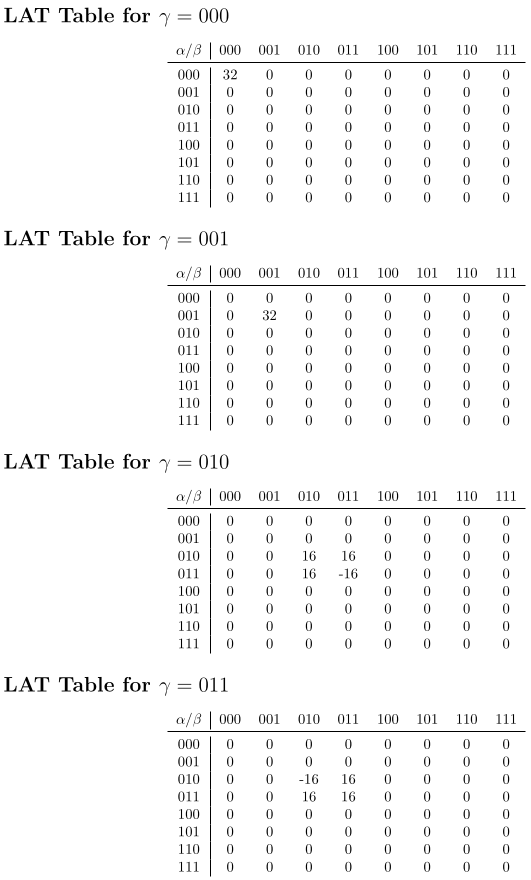
\includegraphics[width=\linewidth]{fig/lat1.png}
  
\end{subfigure}%
\begin{subfigure}{.5\textwidth}
  \centering
  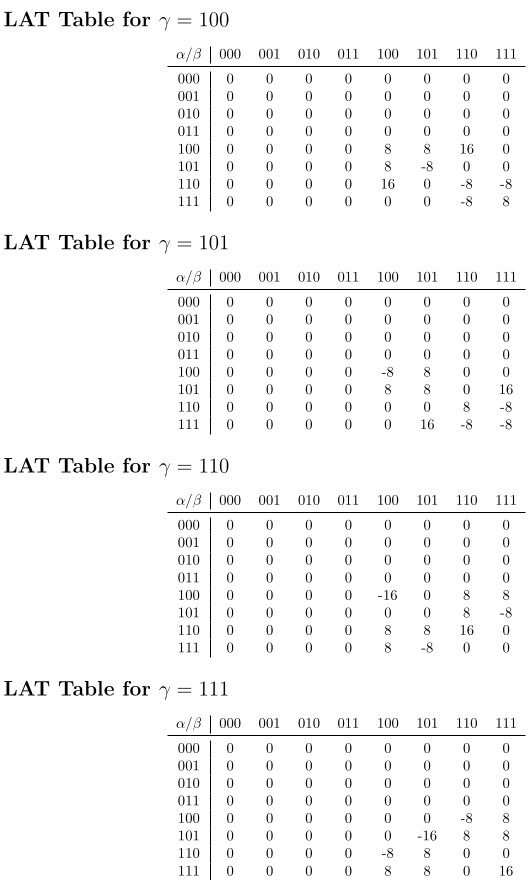
\includegraphics[width=\linewidth]{fig/lat2.png}
  
\end{subfigure}
\caption{LAT of Modular addition $2^3$}
\label{fig:LAT}
\end{figure}

To further improve understanding of linear analysis, some special cases are examined below.


\begin{lemma}
    
Let $\alpha$, $\gamma$, and $\beta$ be masks, and let $z = x \boxplus y$. Then the following equality always holds:

\[
\#\{(x \cdot \alpha) \oplus (y \cdot \beta) = z \cdot \gamma\} = \#\{(x \cdot (\alpha \oplus 1)) \oplus (y \cdot (\beta \oplus 1)) = z \cdot (\gamma \oplus 1)\}
\]
\end{lemma}
\textbf{Sketch of Proof}

Since the bits affecting the LSBs of the masks are not affected by the carry bit, they behave in a balanced manner and do not influence the corresponding entry in the Linear Approximation Table (LAT).

\hfill $\blacksquare$

\vspace{0.2in}

Let us examine some restricted input and output masks.

\vspace{0.1in}

For the equation $z = x \boxplus y$, the best linear approximation is:

\[
z_0 = x_0 \oplus y_0
\]

When the input and output masks are 1, the probability will be 1. Other approximations are not perfect. This approximation is used in attacks on the RC5 \cite{kaliski1995differential} and IDEA \cite{borst1997differential} algorithms.

\vspace{2em}

\begin{theorem}[from \cite{cho2007multiple}]
    If carry bits are considered as a vector, the probability that the XOR of successive bits equals 0 is $3/4$:

    \[
    Pr[\Gamma_{i-1} \cdot C(x,y) = 0] = \frac{3}{4}, \quad i = 1, \dots, 2^{n-1}
    \]
\end{theorem}

\textbf{Proof}

\[
\Gamma_{i-1} \cdot C(x,y) = C_{i-1}(x,y) \oplus C_{i}(x,y) = x_{i}y_{i} \oplus (x_i \oplus y_i \oplus 1)C_{i-1}(x,y)
\]

\vspace{0.1in}

Using the probability that the carry bit is 0:

\[
Pr[\Gamma_{i-1} \cdot C(x,y) = 0] = \frac{3}{4} \cdot \left(\frac{1}{2} + 2^{-i-1}\right) + \frac{3}{4} \cdot \left(\frac{1}{2} + 2^{-i-1}\right) = \frac{3}{4}
\hfill \blacksquare
\]

\vspace{0.2in}

Using this probability, we can say that the probability of $\Gamma_i \cdot (x \boxplus y) = \Gamma_i \cdot (x \oplus y)$ is $3/4$.

\textbf{Proof}

\[
\Gamma_i \cdot (x \boxplus y) = z_i \oplus z_{i+1}
\]
\[
= x_i \oplus y_i \oplus c_i \oplus x_{i+1} \oplus y_{i+1} \oplus c_{i+1}
\]
\[
= \Gamma_i \cdot (x \oplus y) \oplus c_i \oplus c_{i+1}
\]
\[
= \Gamma_i \cdot (x \oplus y) \oplus \Gamma_i \cdot C(x,y)
\]

In this case, the equality $\Gamma_i \cdot (x \boxplus y) = \Gamma_i \cdot (x \oplus y)$ depends on $\Gamma_i \cdot C(x,y)$, and the probability of the equality holding is $3/4$.

\hfill $\blacksquare$

If we select the input and output masks consecutively and equally, the probability will be $3/4$, and the bias will be $1/4$.

\vspace{0.1in}

\begin{example}
    Let $\alpha, \beta, \gamma$ be the input and output masks respectively, and let $\alpha = \beta = \gamma = (0,1,1,0,0)$. In the LAT, the corresponding entry will be 256. Since $\frac{256}{32 \cdot 32} = 1/4$, this indicates the bias.

    To obtain a good bias value, the above-mentioned mask can be used. However, due to factors like shift operations in the rest of the algorithm, which can change the mask, it may not be possible to maintain this mask throughout every round \cite{ashur2016linear}.
    
    \vspace{0.2in}
    
    Suppose there are two consecutive bits in the mask. In this case:
    
    \[
    Pr[\Gamma_{i-1} \cdot C(x,y) = 0] = 3/4, \quad Pr[\Gamma_{i-1} \cdot C(x,y) = 1] = 1/4
    \]
    \[
    Pr[\Gamma_{j-1} \cdot C(x,y) = 0] = 3/4, \quad Pr[\Gamma_{j-1} \cdot C(x,y) = 1] = 1/4
    \]
    
    \vspace{0.1in}
    
    \[
    \Rightarrow Pr[C(x,y)\cdot(\Gamma_{i-1} \oplus \Gamma_{j-1})] = \left(\frac{3}{4} \cdot \frac{3}{4}\right) + \left(\frac{1}{4} \cdot \frac{1}{4}\right) = \frac{5}{8}
    \]
    
    Thus, the bias will be $1/8$. To generalize this situation, we can use the Piling-up Lemma \cite{matsui1993linear}. Let there be $l$ consecutive bits in the mask:
    
    \[
    2^{l-1} \cdot \left(\frac{1}{4}\right)^l
    \]
    
    This will give the bias value.
    

\end{example}

\begin{example}
    Let $\alpha, \beta, \gamma$ be the input and output masks respectively, and let $\alpha = \beta = \gamma = (1,1,0,1,1)$. In the LAT, the corresponding value is 128. Since $\frac{128}{32 \cdot 32} = 1/8$, this indicates the bias.   
\end{example}

To understand the consecutive bits in the mask, we can look at the attack on the SPECK algorithm described in \cite{ashur2016linear}:

\begin{figure}[H]
    \centering
    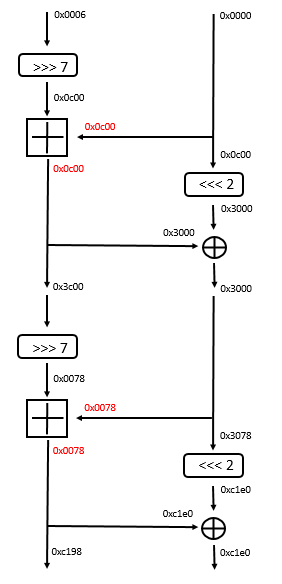
\includegraphics[scale=0.7]{fig/speck.png}
    \caption{2-round linear trail of the SPECK algorithm}
    \label{fig:SPECK}
\end{figure}

Figure \ref{fig:SPECK} shows a 2-round linear trail of the SPECK algorithm. In the first round, since there is 1 consecutive bit in the input and output mask of the modular addition, the bias is $1/4$. In the second round, since there are 2 consecutive bits in the mask, the bias becomes $1/8$.



\section{Modular Addition and Differential Cryptanalysis}

We can start examining the differential analysis of modular addition by constructing its DDT. The only difference when constructing the DDT is that the outputs are not based on an S-box, but rather on the modular sum of two inputs. Pseudo code for constructing modular addition ($2^n$) DDT is given in Algorithm \ref{alg:ddt}.

\begin{algorithm}[H]
    \DontPrintSemicolon
        \For{$0 \leq \alpha < 2^{n}-1$}{
            \For {$0 \leq \beta < 2^{n}-1$}{ 
                \For {$0 \leq x < 2^{n}-1$}{
                    \For{$0 \leq y < 2^{n}-1$}{
                        $z = x \boxplus y$ \\
                        $z^{'} = (x \oplus \alpha) \boxplus (y \oplus \beta)$\\ 
                        \If{$z \oplus z{'} = \gamma$}{
                        $DDT[\alpha][\beta][\gamma]++$
                        }        
                    }
                }    
            }
        }
    \caption{Pseudo code for constructing modular addition ($2^n$) DDT }
    \label{alg:ddt}
\end{algorithm}

Before extending the DDT, let us examine some specific differences.

\vspace{1em}

\noindent
$\pmb{\alpha \boxplus 0 \rightarrow \alpha :}$ When the difference $\alpha$ is given to one of the inputs, we expect to observe the same $\alpha$ difference in the output. Whether this equality holds depends on the number of 1s in the $\alpha$ difference (excluding the most significant bit)~\cite{hong2003differential}.

\vspace{2em}


\begin{example}
    Suppose $x$ and $y$ are 8-bit strings and let $\alpha = (0x42)$.

    \[
    z = x \boxplus y
    \]
    \[
    z^{\prime} = (x \oplus \alpha) \boxplus y
    \]
    
    We analyze the probability Pr$(z \oplus z^{\prime} = \alpha)$. For the condition $z \oplus z^{\prime} = \alpha$ to hold, the equation $z_i \oplus z^{\prime}_i = \alpha_i$ must be satisfied for all $0 \leq i < 7$. Whether this equation holds depends specifically on $i = 2$ and $i = 7$.
    
    As shown in \cite{hong2003differential}, the probability that the equation holds for each bit in the difference (except for the most significant bit) is $\frac{1}{2}$. Therefore,
    \[
    \text{Pr}(z \oplus z^{\prime} = \alpha) = 2^{-2}.
    \]
\end{example}



\subsection{Extension of the Difference Distribution Table for Modular Addition}

In this subsection, we show how the difference distribution table (DDT) of modular addition modulo $2^{m+1}$ can be constructed recursively from the DDT modulo $2^m$. The derivation relies on the dependence of the most significant output difference bit on the carry propagation from lower bit positions.

\subsubsection*{Bit Decomposition}

Let
\[
x = x_m 2^m + x', \qquad
y = y_m 2^m + y',
\]
where $x_m, y_m \in \{0,1\}$ denote the most significant bits (MSBs), and $x', y' \in \{0, \dots, 2^m-1\}$ represent the lower $m$ bits.

Similarly, decompose the input differences as
\[
\Delta x = \alpha 2^m + \Delta x', \qquad
\Delta y = \beta 2^m + \Delta y',
\]
where $\alpha, \beta \in \{0,1\}$ are the MSBs of the input differences.

Define
\[
z = x \boxplus y, \qquad
z^* = (x \oplus \Delta x) \boxplus (y \oplus \Delta y),
\]
and
\[
\Delta z = z \oplus z^* = \gamma 2^m + \Delta z',
\]
where $\gamma \in \{0,1\}$ is the MSB of the output difference.

\subsubsection*{Relation Between the MSB and Carry Bits}

Let
\begin{itemize}
    \item $C_0$ be the carry from the lower $m$ bits of $x \boxplus y$,
    \item $C_1$ be the carry from the lower $m$ bits of $z^*$.
\end{itemize}

The MSBs of the two sums are
\[
z_m = x_m \oplus y_m \oplus C_0,
\]
\[
z_m^* = (x_m \oplus \alpha) \oplus (y_m \oplus \beta) \oplus C_1.
\]

Therefore,
\[
\gamma = z_m \oplus z_m^*,
\]
which yields
\begin{equation}
\gamma = (\alpha \oplus \beta) \oplus (C_0 \oplus C_1).
\label{eq:msb_relation}
\end{equation}

Equation~\eqref{eq:msb_relation} is the fundamental relation governing the extension of the DDT. The MSB of the output difference depends only on the XOR of the MSBs of the input differences and the parity of the carry bits from the lower part.

\subsubsection*{Partition of the Base DDT}

Consider the DDT of addition modulo $2^m$. Each entry corresponds to a triple $(\Delta x', \Delta y', \Delta z')$.

We partition this DDT into two disjoint subsets according to the carry parity:
\[
v := \{ (\Delta x', \Delta y', \Delta z') : C_0 \oplus C_1 = 0 \},
\]
\[
u := \{ (\Delta x', \Delta y', \Delta z') : C_0 \oplus C_1 = 1 \}.
\]

Thus,
\[
\mathrm{DDT}_{2^m} = u \cup v.
\]

\subsubsection*{Construction of the Extended DDT}

From Equation~\eqref{eq:msb_relation}, two cases arise.

\paragraph{Case 1: $\gamma = 0$}

Equation~\eqref{eq:msb_relation} becomes
\[
C_0 \oplus C_1 = \alpha \oplus \beta.
\]

Hence:
\begin{itemize}
    \item If $\alpha \oplus \beta = 0$, the contribution comes from $v$.
    \item If $\alpha \oplus \beta = 1$, the contribution comes from $u$.
\end{itemize}

Since extending from $m$ to $m+1$ bits introduces four combinations of $(x_m, y_m)$, each valid entry of the base DDT is replicated four times. Therefore, the upper half of the extended DDT corresponding to $\gamma = 0$ has block structure
\[
\begin{bmatrix}
4v & 4u \\
4u & 4v
\end{bmatrix}.
\]

\paragraph{Case 2: $\gamma = 1$}

Now Equation~\eqref{eq:msb_relation} becomes
\[
C_0 \oplus C_1 = \alpha \oplus \beta \oplus 1.
\]

Thus:
\begin{itemize}
    \item If $\alpha \oplus \beta = 0$, the contribution comes from $u$.
    \item If $\alpha \oplus \beta = 1$, the contribution comes from $v$.
\end{itemize}

The lower half of the extended DDT therefore has block structure
\[
\begin{bmatrix}
4u & 4v \\
4v & 4u
\end{bmatrix}.
\]

\subsubsection*{Impossibility Regions}

Certain combinations of $(\gamma, C_0 \oplus C_1)$ lead to contradictions.

\paragraph{Example: $\gamma = 0$ and $C_0 \oplus C_1 = 1$ in the region $\alpha=\beta=0$}

From Equation~\eqref{eq:msb_relation}:
\[
0 = 0 \oplus (C_0 \oplus C_1),
\]
which implies
\[
C_0 \oplus C_1 = 0.
\]

Thus, the assumption $C_0 \oplus C_1 = 1$ is impossible. A complete case analysis over all assignments of $(x_m, y_m)$ confirms that the carry bits on both sides are always equal. Consequently, the corresponding region of the DDT contains only zero entries.

\paragraph{Symmetric Case}

Similarly, for
\[
\gamma = 1 \quad \text{and} \quad C_0 \oplus C_1 = 0
\]
in the region $\alpha=\beta=1$, Equation~\eqref{eq:msb_relation} forces
\[
C_0 \oplus C_1 = 1,
\]
which is a contradiction. Hence, this region is also impossible.

\subsubsection*{Recursive Structure of the DDT}

Combining all cases, the DDT modulo $2^{m+1}$ can be expressed recursively as
\[
\mathrm{DDT}_{2^{m+1}} =
\begin{bmatrix}
A & B \\
B & A
\end{bmatrix},
\]
where the blocks $A$ and $B$ are scaled versions of $u$ and $v$ determined by carry parity.

This demonstrates that the DDT of modular addition exhibits a self-similar recursive structure. The extension from $m$ to $m+1$ bits is completely governed by the parity of the carry bits from the lower part of the addition.

The complete block-wise construction of the extended DDT is illustrated in Figure~\ref{fig:uuvv1}.


\begin{figure}[h]
    \centering
    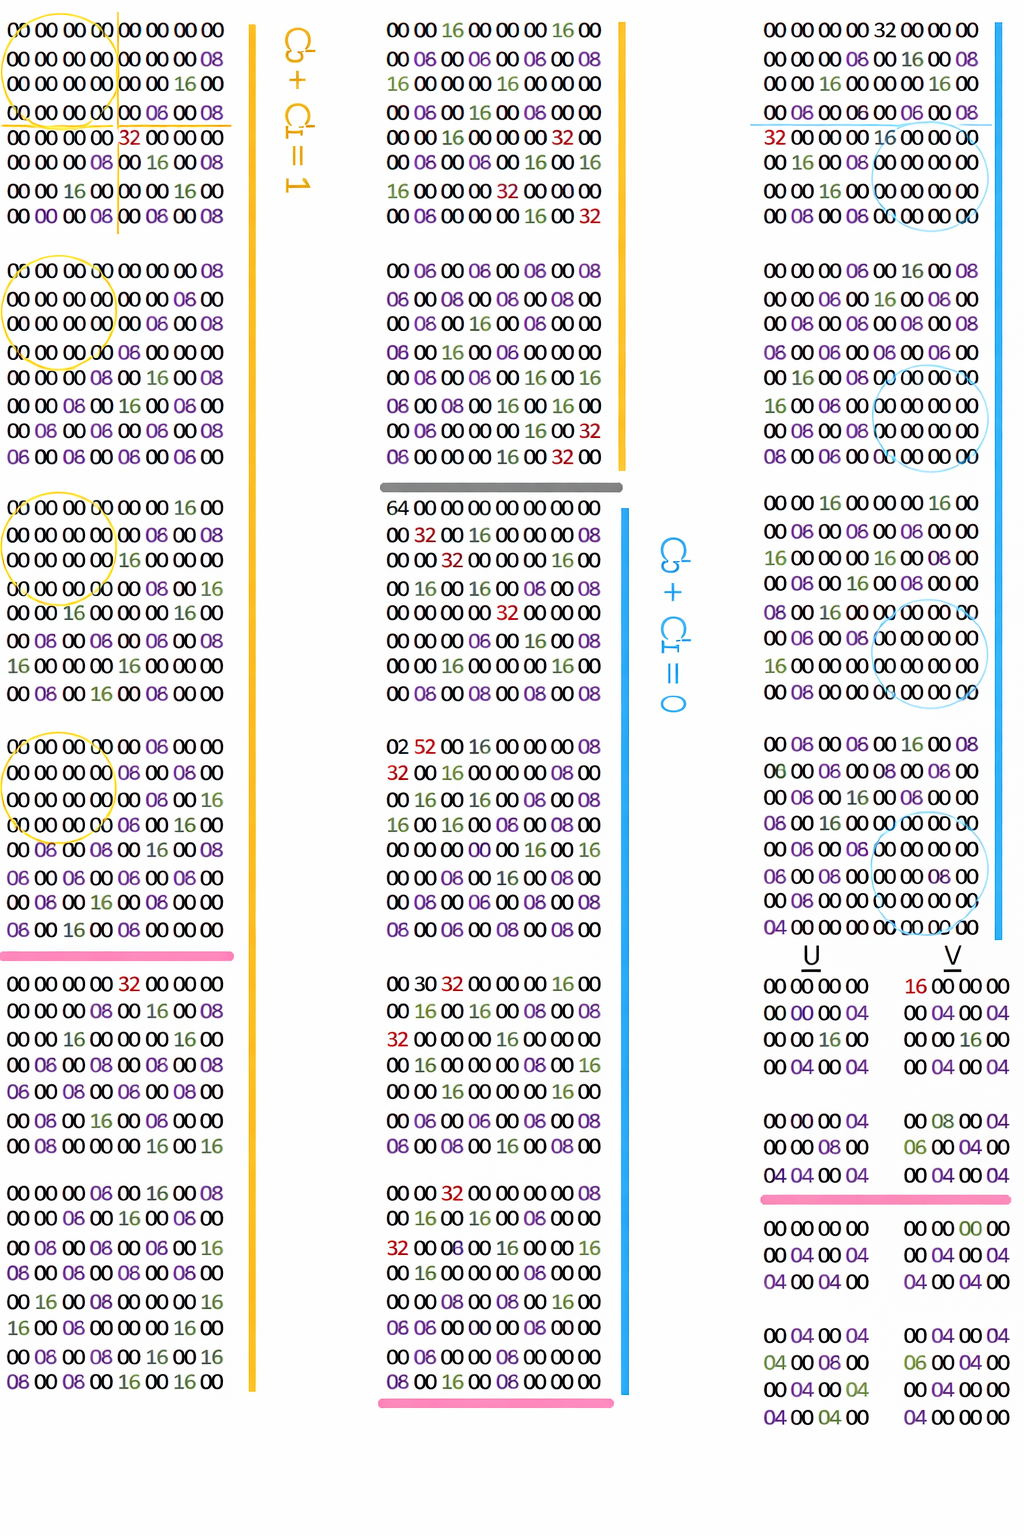
\includegraphics[width = 14cm]{fig/uuvv1.png}
    \caption{DDT extension method results}
    \label{fig:uuvv1}
\end{figure}



\section{Conclusion}
This paper has presented a detailed analysis of modular
addition from a cryptanalytic perspective, focusing on both
linear and differential approaches. We have demonstrated
how the probability distribution of carry bits affects linear
approximations and shown methods for constructing LAT and
DDT tables specifically for modular addition operations.
Our analysis reveals that the probability of carry bits ap-
proaches 1/2 as the bit position increases, which has significant
implications for linear cryptanalysis. We have also shown how
to extend DDTs for larger bit sizes by leveraging smaller tables
and carry bit relationships.
These findings provide valuable tools for cryptanalysts
examining algorithms that use modular addition and offer
insights for cipher designers to strengthen their constructions
against these types of attacks.

\newpage

\printbibliography

\end{document}